\documentclass{article}


\usepackage{mathrsfs}
\usepackage{amsthm,amsmath,amssymb,bbm}
\usepackage{natbib}
\usepackage{multirow}
\usepackage{subfigure}
\usepackage{makecell}
\usepackage{booktabs}
\usepackage{array}
\usepackage{MnSymbol}
%\usepackage{fullpage}
\usepackage{url}
\usepackage{algorithm}
\usepackage{algorithmic}
\usepackage{bm}
%\usepackage{mathtools}
\usepackage{wrapfig}
\usepackage{lipsum}
\usepackage{mathrsfs}
\usepackage{graphicx}
\graphicspath{ {/Users/Cindy/Documents/images/} }
\usepackage{dsfont}
\usepackage{titling}
\usepackage{mathtools}
\usepackage{amsmath,lipsum}
\newcommand{\mypm}{\mathbin{\smash{%
\raisebox{0.35ex}{%
            $\underset{\raisebox{0.5ex}{$\smash \frown$}}{\smash \smile}$%
            }%
        }%
    }%
}

\newcommand{\tlarge}{\mathbin{\smash{%
\raisebox{0.35ex}{%
            $\underset{\raisebox{0.5ex}{$\smash \sim$}}{\smash >}$%
            }%
        }%
    }%
}

\newcommand{\tsmall}{\mathbin{\smash{%
\raisebox{0.35ex}{%
            $\underset{\raisebox{0.5ex}{$\smash \sim$}}{\smash <}$%
            }%
        }%
    }%
}

%\usepackage{datetime}
%\usepackage{epstopdf,mathabx}

%\usepackage{algcompatible}
%\pagestyle{fancy}
%\lhead{Semiparametric Spjiu arse Column Inverse Operator}
%\rhead{  }
%%\cfoot{center of the footer!}
%\renewcommand{\headrulewidth}{1pt}
%\renewcommand{\footrulewidth}{1pt}
\usepackage{multirow}
%\usepackage{subfigure}
%\usepackage{makecell}

\usepackage[usenames,dvipsnames,svgnames,table]{xcolor}
\usepackage[colorlinks,
linkcolor=red,
anchorcolor=blue,
citecolor=blue
]{hyperref}

\def\T{{ \mathrm{\scriptscriptstyle T} }}

\def\skeptic{{\sc skeptic}}
\newcommand{\sgn}{\mathop{\mathrm{sign}}}
\providecommand{\norm}[1]{\|#1\|}
\providecommand{\bnorm}[1]{\big\|#1\big\|}
\providecommand{\enorm}[1]{| \! | \! |#1| \! | \! |}
\providecommand{\bemnorm}[1]{\big| \! \big| \! \big|#1\big| \! \big| \! \big|}

\newcommand*{\expect}{\mathsf{E}}
\newcommand*{\prob}{\mathsf{P}}
\newcommand\Tau{\mathcal{T}}


%\numberwithin{equation}{section}
%\numberwithin{thm}{section}
%\numberwithin{asmp}{section}
%\numberwithin{defn}{section}
%\numberwithin{figure}{section}
%\numberwithin{table}{section}
%\numberwithin{rem}{section}



%%%%My macros

\newcommand*{\Sc}{\cS^{\perp}}
\newcommand*{\Ac}{\cA^{\perp}}
\newcommand*{\supp}{\mathrm{supp}}
%\usepackage{cite}

\newcommand \rF{\mathrm{F}}
\newcommand \rd{\mathrm{d}}
\newcommand \ru{\mathrm{u}}
\newcommand \rv{\mathrm{v}}
\newcommand \rw{\mathrm{w}}
\newcommand \rwb{\bm{\mathrm{w}}}
\newcommand{\e}{\mathbb{E}}
\newcommand{\nn}{\nonumber}
\newcommand{\nb}[1]{{\bf\color{blue} [#1]}}
\newcommand{\nr}[1]{{\bf\color{red} [#1]}}

%%%%%%%%%%%
\newcommand \btt{\bbeta}
\newcommand \hbt{\hat{\btt}}
\newcommand \bttc{\bbeta^*}
\newcommand \tbs{\tilde{\btt}^*}
\newcommand \tbt{\tilde{\btt}}
\newcommand \mbu{\ub}

%%%%Definition of new notations
\newcommand{\FDP}{{\rm FDP}}
\newcommand{\thh}{-{{\rm th}}}


%%%%Definition of Equation environment
\def\##1\#{\begin{align}#1\end{align}}
\def\$#1\${\begin{align*}#1\end{align*}}

%%%%Definition of Operators
\newcommand {\vecc}{\textnormal {vec}}
\newcommand {\cov}{\textnormal {cov}}
\newcommand {\var}{\textnormal {var}}

\def\T{\mathrm{\scriptstyle T}} %%%transpose operator
\def\sn{\sum_{i=1}^n}
\newcommand {\summ}{\textnormal {sum}}

\newcommand {\F}{\textnormal {F}}
\newcommand\X{\mathrm{X}}
\newcommand\Y{\mathrm{Y}}
\newcommand\E{\mathrm{E}}
\newcommand\V{\mathrm{V}}
\newcommand\U{\mathrm{U}}
\newcommand\W{\mathrm{W}}


%%%%Definition of Roman Numbers
\newcommand{\Rom}[1]{\text{\uppercase\expandafter{\romannumeral #1\relax}}}


%\addtolength{\textwidth}{1in} \addtolength{\oddsidemargin}{-0.5in}
%\addtolength{\textheight}{1in} \addtolength{\topmargin}{-0.62in}
%margin and textwidth
\usepackage{geometry}
 \geometry{
 a4paper,
 %total={170mm,257mm},
 left=28mm,
 top=30mm,
 }
\textwidth=6in

\renewcommand{\baselinestretch}{1.1}

\usepackage{mathtools}
\DeclarePairedDelimiter\ceil{\lceil}{\rceil}
\DeclarePairedDelimiter\floor{\lfloor}{\rfloor}

\usepackage{enumitem}

\usepackage[latin1]{inputenc}
\usepackage{tikz}
\usetikzlibrary{shapes,arrows}
\usepackage{Sweave}
\begin{document}
\Sconcordance{concordance:report.tex:report.Rnw:%
1 176 1 1 0 315 1}


\graphicspath{ {GA/} }

\title{\LARGE Genetic Algorithm-R Package Final Report}
\author{David Chen, Qi Chen, Emily Suter and Xinyi(Cindy) Zhang}


\date{\today}

\maketitle

\begin{abstract}
Genetic Algorithm (GA) is a search-based optimization technique based on the principles of Genetics and Natural Selection. It is frequently used to find optimal or near-optimal solutions to difficult problems which otherwise would take a lifetime to solve. In this report, we will first introduce how we set up the genetic algorithm and the main steps. We then describe the testing procedure carried out. In section \ref{s3}, we include the results from the example we have taken to apply our GA algorithm. Contributions of each team member is collected in the last part, section \ref{s4}.
\end{abstract}

\begin{center}
\textbf{Github Username:} dchen49
\end{center}

\newpage
\pagestyle{empty}

\section{Introduction to Our Genetic Algorithm}\label{s1}

Our package is comprised of 4 major functions: \textit{select()}, \textit{regress()}, \textit{mate()}, and \textit{evolve()}.\\

\textit{select()} is the main, exported function which takes in all user arguments and wraps all other functions. \textit{select()} also loops over generations, checks stopping criteria, and creates the output list object with 4 components: \textit{optimum}, \textit{fitPlot}, \textit{fitStats}, and \textit{GA}. \textit{optimum} contains the names of the selected variables, the fitness value achieved, and the regression object. \textit{fitPlot} is a ggplot of the mean, median, and maximum fitness per generation and is generated from the table in \textit{fitStats}. \textit{GA} contains the elite subset of genotypes and all fitness values for each generation.\\

\textit{regress()} calculates the fitness of the regresssion model using a particular group of covariates and returns fitness metric as a single number to be maximized. In our GA implementation, \textit{regress()} is called in an apply loop to operate over the entire genotype poulation and return a vector of fitness values.\\

\textit{mate()} selects parents using one of 4 selection methods: tournament selection, linear ranking selection, exponential ranking selection, or roulette wheel selection. Each method is defined as a sub-function which is then called by \textit{mate()}. The output is a genotype population of parents to be passed into \textit{evolve()}.\\

\textit{evolve()} performs crossing-over of genotypes and mutates single alleles by calling subfunctions \textit{singlecrossover()}, \textit{multiplecrossover()}, and \textit{mutate()}. It returns a population of altered genotypes to be combined with elite survivors to produce the next generation.\\
\\
To better introduce our genetic algorithm, the following Figure \ref{p1} diagrams the workflow

\vspace{5mm}

% Define block styles
\tikzstyle{decision} = [diamond, draw, fill=blue!20,
    text width=4.5em, text badly centered, node distance=3cm, inner sep=0pt]
\tikzstyle{block} = [rectangle, draw, fill=blue!20,
    text width=5em, text centered, rounded corners, minimum height=4em]
\tikzstyle{bblock} = [rectangle, draw, fill=blue!20,
    text width=8em, text centered, rounded corners, minimum height=4em]
\tikzstyle{line} = [draw, -latex']
\tikzstyle{cloud} = [draw, ellipse,fill=red!20, node distance=3cm, text width=5em,
    rounded corners, minimum height=3em]
\tikzstyle{begin} = [rectangle, draw, fill=green!20,
    text width=8em, text centered, rounded corners, minimum height=4em]

\begin{tikzpicture}[node distance = 2cm, auto]\label{p1}
    % Place nodes
    \node [begin] (init) {Algorithm Start: Initialize P$_{0}$};
    \node [block, below of=init, node distance=3cm] (evaluate) {Compute Fitness};
    \node [decision, below of=evaluate] (decide) {Checking Stopping Criteria?};
    \node [cloud, right of=decide, node distance=4.5cm] (stop) {Terminate and return the best!};
    \node [bblock, left of=evaluate, node distance=5.5cm] (update) {Recombine with survivors from the last generation};


    \node [block, below of=decide, node distance=3cm] (continue) {Parents Selection};
    \node [block, left of=continue, node distance=5.5cm] (continuea) {Offspring Generation};
    % Draw edges
    \path [line] (init) -- (evaluate);
    \path [line] (evaluate) -- (decide);
    %\path [line] (decide) -| node [near start] {no} (update);
    \path [line] (update) -- node {new population}(evaluate);
    \path [line] (decide) -- node {no}(continue);
    \path [line] (continue) -- node {Evolution}(continuea);
    \path [line] (decide) -- node {yes}(stop);
    \path [line] (continuea) --  node {step into} (update);


\end{tikzpicture}

\section{Testing}\label{s2}
We have tested the input and output format for each individual functions in our GA algorithm, as well as the stopping criteria. To test the function select() as a whole, we tested its ability to find max fitness using lm/glm and AIC/BIC on a manufactured dataset.\\

\noindent
To investigate whether our GA algorithm can attain the same optimum as global search for all possible genotypes, we create another dataset to test this. We generated the data as follows:

\vspace{3mm}
\noindent
Consider number of variables $p=5$, and we generate covariates $X=(X_{1}, \cdots, X_{5})^{\T}$ from different distributions, where $X_{1}\sim N(0,25)$, $X_{2}\sim \mathrm{Unif}(0,1)$, $X_{3}\sim \mathrm{Poisson}(1)$, $X_{4}\sim \mathrm{exp}(2)$, $X_{5}\sim \mathrm{Gamma}(10,1)$. The responses $Y$ are generated by simply averaging $X_{1}$ and $X_{3}$, i.e. $Y=\frac{X_{1}+X_{3}}{2}$. Apart from finding optimal genotype via Genetic Algorithm, we also compute all the fitness values for all 32 genotypes to see what the exact global optimum is and thus the "best" genotype. Since the reponse $Y$ is only related to variables $X_{1}$ and $X_{3}$, we hope that both the global search approach and the GA algorithm can only select these two features but not others. Additionally, we also hope that the results returned by these two methods are consistent. Comparison results are presented below in Table \ref{table:1}.


\begin{table}[htp]
    \centering
    \caption{Comparison of optimal fitness values with respect to global search and GA algorithm}
    \vspace{0.05in}
            \newsavebox{\tableboxb}
\begin{lrbox}{\tableboxb}
    \begin{minipage}{.5\linewidth}
      \caption{Global Search}
      \centering
        \begin{tabular}{c|c|c}
  \hline
 & AIC & BIC \\
  \hline
lm & 19963.50 & 19945.41 \\
  glm & 20175.50 & 20160.68 \\
   \hline
\end{tabular}
    \end{minipage}%
    \begin{minipage}{.5\linewidth}
      \centering
       \caption{GA Algorithm}
        \begin{tabular}{r|r|r}
  \hline
 & AIC & BIC \\
  \hline
lm & 19963.50 & 19945.41 \\
  glm & 20175.50 & 20160.68 \\
   \hline
\end{tabular}
    \end{minipage}
    \end{lrbox}
    \label{table:1}
\scalebox{1}{\usebox{\tableboxb}}
\end{table}


\noindent
One can see from the results in Table \ref{table:1} that for each combination of fitted model and fitness criteria, the GA algorithm and global search method give exactly the same results. In other words, our GA algorithm does find the global maximum fitness value, i.e global minimum value for AIC or BIC.

\vspace{3mm}
\noindent
Next, we present the genotypes returned by both global search and GA algorithm in Table \ref{table:4}.

\begin{table}[htp]
    \centering
    \caption{Comparison of optimal fitness values with respect to global search and GA algorithm}
    \vspace{0.05in}
            \newsavebox{\tableboxc}
\begin{lrbox}{\tableboxc}
    \begin{minipage}{.5\linewidth}
      \caption{Global Search}
      \centering
       \begin{tabular}{r|l|l}
  \hline
 & AIC & BIC \\
  \hline
lm & 11100 & 10100 \\
  glm & 10100 & 10100 \\
   \hline
\end{tabular}
    \end{minipage}%
    \begin{minipage}{.5\linewidth}
      \centering
        \caption{GA Algorithm}
        \begin{tabular}{r|l|l}
  \hline
 & AIC & BIC \\
  \hline
lm & 11100 & 10100 \\
  glm & 10100 & 10100 \\
   \hline
\end{tabular}
    \end{minipage}
    \end{lrbox}
    \label{table:4}
\scalebox{1}{\usebox{\tableboxc}}
\end{table}

\noindent
In summary, our GA algorithm can find the global optima, results of which are consistent with that from global search.


\section{Application}\label{s3}
In this section, we considered two applications of our genetic algorithm, one on the dataset generated from a linear regression model, which aims to evaluate whether the designed algorithm can successfully select those important features, given known relevant variables combined with some noise terms. Another application is based on the baseball data collected from the textbook ``Computational Statistics'' \citet{compute}. Details will be illustrated as follows.

\subsection{Application on Data Generated from Linear Regression Model}
In this section, we will first introduce how we generate the covariates and responses for evaluating our genetic algorithm on feature selection. We first generate covariates from the multivariate normal distribution $N_{p}(\bm{0}, \Sigma_{x})$, where the $(j, j^{\prime})$ entry of $\Sigma_{x}$ satisfies
$$
\Sigma_{x(j,j^{\prime})} = 0.5^{|j-j^{\prime}|}, \mbox{ for } 1\leq j, j^{\prime}\leq p.
$$
Setting sample size $n=300$ and feature dimension $p=10$, we then fit the linear regression model
$$
Y = X\beta,
$$
where $\beta=(\beta_{1}, \cdots, \beta_{6})^{\mathrm{T}}$ is generated from univariate normal distribution $N(3, 25)$. Moreover, we add some noise $\epsilon=(\epsilon_{1}, \cdots, \epsilon_{n})$ to the covariates generated as above. $\epsilon_{i}$, for $1\leq i \leq n$, is generated from $N_{20}(\bm{0}, \Sigma_{x})$, which has the same parameter setting as $X$ except the dimension. We then combine $X$ and the noise terms together. The resulting covariates matrix is given by
$$
\tilde{X} = (X|\epsilon).
$$
Apply our genetic algorithm to fit a linear model regressing $Y\in \mathbb{R}^{n}$ on $\tilde{X}\in \mathbb{R}^{n\times 30}$. Given $10$ relevant covariates and 20 noise terms, the designed GA algorithm gives the following results for feature selection. Results are presentesd in Table: \ref{t1}
\begin{table}[ht]
\centering
\caption{Selected Genotypes}
\resizebox{\columnwidth}{!}{%
\begin{tabular}{rrrrrrrrrrrrrrrrrrrrrrrrrrrrrrr}
  \hline
Var & x1 & x2 & x3 & x4 & x5 & x6 & x7 & x8 & x9 & x10 & n1 & n2 & n3 & n4 & n5 & n6 & n7 & n8 & n9 & n10 & n11 & n12 & n13 & n14 & n15 & n16 & n17 & n18 & n19 & n20 \\
  \hline
Gene & 1 & 1 & 1 & 1 & 1 & 1 & 1 & 1 & 1 & 1 & \textcolor{red}{1} & \textcolor{red}{1} & 0 & \textcolor{red}{1} & \textcolor{red}{1} & 0 & \textcolor{red}{1} & 0 & \textcolor{red}{1} & 0 & \textcolor{red}{1} & 0 & \textcolor{red}{1} & 0 & \textcolor{red}{1} & \textcolor{red}{1} & \textcolor{red}{1} & \textcolor{red}{1} & \textcolor{red}{1} & \textcolor{red}{1} \\
   \hline
\end{tabular}%
}\label{t1}
\end{table}

One can see that our GA algorithm can select all the relevant features, but will also include some irrelevant noise terms denoted in red. Next, we will take a look at the coefficients of those noise terms from the regression model and further investigate whether the "noise" terms are significant or not. Results are presented in Table \ref{Table:8} and Table \ref{Table:9}.

\vspace{3mm}
\noindent

Coefficients of Relevant Variables:
\begin{table}[ht]
\centering
\caption{x-variables}
\begin{tabular}{r|r|r|r|r|r|r|r|r|r}
  \hline
 x1 & x2 & x3 & x4 & x5 & x6 & x7 & x8 & x9 & x10 \\
  \hline
8.70 & 0.98 & 8.46 & -0.74 & 1.87 & -1.31 & 5.47 & 5.07 & 0.61 & 4.99 \\
   \hline
\end{tabular}\label{Table:8}
\end{table}

\noindent
Coefficients of Noise terms:
\begin{table}[ht]
\centering
\caption{n-Noise terms}
\resizebox{\columnwidth}{!}{%
\begin{tabular}{r|r|r|r|r|r|r|r|r|r|r|r|r|r|r}
  \hline
 n1 & n2 & n3 & n4 & n5 & n7 & n9 & n11 & n13 & n15 & n16 & n17 & n18 & n19 & n20 \\
  \hline
3e-15 & -4e-15 & -2e-15 &4e-15& -2e-15& -1e-15& -5e-15 &5e-15& -1e-15& 1e-15& 5e-15& -1e-14& 4e-15& -5e-15& 3e-16 \\
   \hline
\end{tabular}%
}\label{Table:9}
\end{table}

\noindent
One can see from the table that although we have included some noise terms, but values of those coefficients are quite small, which indicates that these noise terms are not significant.

We then repeated the previously described variable selection $ 50 $ times. Figure \ref{Figure: 1} plots the summed absolute value of the coefficients for all selected variables. One can clearly see the same pattern described previously, where the weights of the noise terms are negligible compared to those of the valid x terms.

\begin{figure}
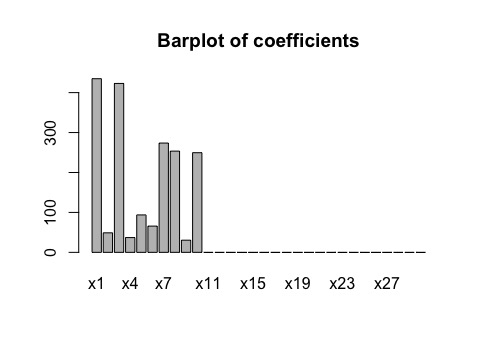
\includegraphics{barplot}
\caption{Summed Weights of Regression Variables}
\label{Figure: 1}
\end{figure}


% \vspace{3mm}
% \noindent
% A plot monitoring the optmization process is also included:
% \begin{figure}[h]
% \caption{How it evolves}
% \centering
% \includegraphics[width=10cm, height=6cm]{r2}
% \end{figure}

\subsection{Application on Baseball Data}
We next test our genetic algorithm on a real data set to demonstrate the ability to select an optimal variable subset.  A data set of baseball player statistics and salary numbers was obtained via the website for \citet{compute}.

The data set contains 27 different statistics (such as hits and on-base percentage) for 337 players in the 1991 baseball season.  Additionally, the data set contains the salaries for the same 337 players in the 1992 season.  We used our genetic algorithm to select player statistic(s) that most influence that players salary in the following year.

We tested our algoritms performance on combinations of different fitness criteria (AIC, BIC) and selection method (tournament, exponential ranking, linear ranking, roulette wheel).  All other input parameters were held constant at maxGen = 500, minGen = 50, population = 500, pMutate = 0.1, crossParams = c(0.8, 1), and  eliteRate = 0.1.  The fitness values are shown in Table \ref{table:7}.

\begin{table}[htp]
    \centering
    \caption{Maximum Fitness Value}

\begin{tabular}{ |c|c|c|c|c|  }

 \hline
 Selection Method & LM, AIC & LM, BIC & GLM, AIC & GLM, BIC\\
 \hline
 Tournament &  5376.012   & 5409.318 & 5375.850  & 5412.395\\
 Linear & 5376.354 & 5409.318  & 5375.850 & 5409.318\\
 Exponential & 5378.926 & 5414.315 & 5379.316 & 5422.321\\
 Roulette   & 5376.365 & 5417.421 & 5376.353 & 5417.723\\
 \hline
\end{tabular}
    \label{table:7}
\end{table}

\vspace{5cm}

In this simulation, the minimum (i.e., best) fitness value was produced using GLM as the model, AIC as the fitness criteria, and tournament or linear ranking as the selection method.  Generally, the difference between AIC and BIC was greater than the variance across selection methods.

The exponential ranking selection method converged the fastest, followed by tournament selection, as shown in Table \ref{table:8}.

\begin{table}[htp]
    \centering
    \caption{Iterations to Reach Maximum Fitness Value}

\begin{tabular}{ |c|c|c|c|c|  }
 \hline
 Selection Method & LM, AIC & LM, BIC & GLM, AIC & GLM, BIC\\
 \hline
 Tournament & 64  & 69 & 62  & 63\\
 Linear & 75 & 96  & 80 & 88\\
 Exponential & 53 & 52 & 53 & 53\\
 Roulette   & 84 & 85 & 94 & 111\\
 \hline
\end{tabular}

    \label{table:8}
\end{table}


In general, the top genotype returned when using BIC fitness criteria had fewer variables than those using AIC.  This makes sense since BIC has a greater penalty for higher numbers of variables:  with AIC, the penalty is \textit{2p}, whereas with BIC the penalty is \textit{ln(n)p}.


The number of variables returned in the best genotype of each combination is shown in Table \ref{table:9}.

\begin{table}[htp]
    \centering
    \caption{Number of Variables in Best Genotype}

    \begin{tabular}{ |c|c|c|c|c|  }
      \hline
      Selection Method & LM, AIC & LM, BIC & GLM, AIC & GLM, BIC\\
      \hline
      Tournament &  10   & 6 & 12  & 6\\
      Linear & 10 & 7  & 15 & 6\\
      Exponential & 11 & 7 & 16 & 8\\
      Roulette   & 14 & 7 & 14 & 7\\
    \hline
    \end{tabular}

    \label{table:9}
\end{table}

Regardless of method, model, or criteria, Strength of Schedule (\textit{sos}), Runs Batted In (\textit{rbis}), Free Agency (\textit{freeagent}), and Arbitration (\textit{arbitration}) are all included in the top genotypes.  Free Agency and Arbitration had very high regression coefficients, hovering around 1300 and 850, respectively; conversely, the coefficients of RBIs and SOS were much lower, about 25 and -12.  We hypothesize that this is because a player that becomes a free agent and gets signed to a new team will likely negotiate a large salary contract with their new team;  players that enter free agency and don't get signed aren't included in this data set.



\section{Group Member Contributions}\label{s4}
David Chen:

\vspace{3mm}
\noindent
Qi Chen:

\vspace{3mm}
\noindent
Emily Suter:

\vspace{3mm}
\noindent
Xinyi(Cindy) Zhang:

\nocite{selection}
\bibliographystyle{ims}
\bibliography{243project}



\end{document}
